%-B--------------------------------------------------------------------------B-%
\begin{frame}[allowframebreaks]
\frametitle{Définitions}


\begin{itemize} \itemsep0.8em
    \item un \textbf{corpus} est un ensemble de documents (textes, images, 
          vidéos) regroupés dans une optique précise
    \item dans le cadre de ce cours~: \alert{\fbox{corpus $\to$ textes}}
    \item caractéristiques d'un corpus:
    \begin{itemize}
        \item la taille
        \item le langage
        \item le temps couvert par les textes du corpus
        \item le registre de langage
    \end{itemize}
\end{itemize}

\framebreak


\begin{itemize} \itemsep0.8em
    \item le corpus doit atteindre une \textbf{taille} critique pour permettre 
          des traitements statistiques fiables
    \begin{itemize}
        \item 10K+ phrases pour entraîner un \textit{POS-tagger}
        \item 20M+ mots pour construire un modèle de langue
    \end{itemize}
    \item un corpus \textbf{monolingue} couvre une seule langue, et une seule 
          déclinaison de cette langue
    \begin{itemize}
        \item e.g.~français de France et français du Québec
    \end{itemize}
\end{itemize}

\framebreak

\begin{itemize} \itemsep0.8em
    \item la \textbf{période couverte} par les textes doit être courte
    \begin{itemize}
        \item français d'aujourd'hui $\ne$ français parlé au 19$^e$ siècle
        \item français d'aujourd'hui $\ne$ français de 1990 (néologismes)
    \end{itemize}
    \item les \textbf{registres de langage} doivent être séparés
    \begin{itemize}
        \item un corpus de textes scientifiques ne peut être utilisé pour 
              extraire des informations sur les textes vulgarisés
        \item un corpus de textes scientifiques et vulgarisés ne permettra pas 
              de tirer de conclusion sur ces deux registres
    \end{itemize}
\end{itemize}

\end{frame}
%-E--------------------------------------------------------------------------E-%

% %-B--------------------------------------------------------------------------B-%
% \begin{frame}
% \frametitle{Les différents types de corpora}
% \tableofcontents[sectionstyle=show/hide,subsectionstyle=show]
% \end{frame}
% %-E--------------------------------------------------------------------------E-%


%==============================================================================%
\subsection{Corpus parallèle}
%==============================================================================%


%-B--------------------------------------------------------------------------B-%
\begin{frame}
\frametitle{Corpus parallèle}

\begin{itemize} \itemsep0.8em
    \item un \textbf{corpus parallèle} est un ensemble de paires de textes tel 
          que, pour une paire, un des textes est la traduction de l'autre
    \item un \textbf{alignement} des unités textuelles est nécessaire:
    \begin{itemize}
        \item mettre en correspondance des unités textuelles en langue source
              avec celles de la langue cible
    \end{itemize}
    \item un alignement peut être manuel ou automatique
    \item la granularité de l'alignement dépend de l'utilisation
    \begin{itemize}
        \item traduction automatique, dictionnaires bilingues, etc.
    \end{itemize}
\end{itemize}

\end{frame}
%-E--------------------------------------------------------------------------E-%

%-B--------------------------------------------------------------------------B-%
\begin{frame}[shrink=5]
\frametitle{Alignement de phrases}

\vspace*{1em}

\small

\begin{columns}[c] 
    
    \column{.45\textwidth}

    Il s'agit de l'un des sauropodes les plus connus. \\[0.5em]

    C'était un très grand quadrupède au long cou, avec une longue queue en 
    forme de fouet.\\[0.5em]

    Ses membres antérieurs étaient légèrement plus courts que ses membres 
    postérieurs, ce qui lui donnait une posture horizontale.\\[1.2em]
    ~

    \column{.1\textwidth}

    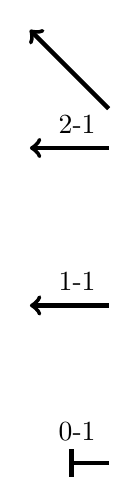
\begin{tikzpicture}
        \draw [ultra thick, <-] (0,5.5) -- (1,4.5);
        \draw [ultra thick, <-] (0,4) -- (1,4);
        \node at (0.6,4.3) {2-1};
        \draw [ultra thick, <-] (0,2) -- (1,2);
        \node at (0.6,2.3) {1-1};
        \draw [ultra thick,|-] (0.5,0) -- (1,0);
        \node at (0.6,0.4) {0-1};
    \end{tikzpicture}
    \vspace*{1em}

    \column{.45\textwidth}

    One of the best-known sauropods, Diplodocus was a very large long-necked 
    quadrupedal animal, with a long, whip-like tail.\\[1.2em]

    Its forelimbs were slightly shorter than its hind limbs, resulting in a 
    largely horizontal posture.\\[1.2em]

    It is the longest dinosaur known from a complete skeleton.

\end{columns}

\end{frame}
%-E--------------------------------------------------------------------------E-%


%-B--------------------------------------------------------------------------B-%
\begin{frame}[shrink=5]
\frametitle{Alignement de mots}

\vspace*{1em}

\begin{center}
Je suis Français . \\
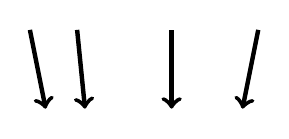
\begin{tikzpicture}
    \draw [ultra thick, <-] (0.4,0) -- (0.2,1);
    \draw [ultra thick, <-] (0.9,0) -- (0.8,1);
    \draw [ultra thick, <-] (2,0) -- (2,1);
    \draw [ultra thick, <-] (2.9,0) -- (3.1,1);
\end{tikzpicture}\\[-0.2em]
I am French .
\end{center}

\vspace*{0.5em}

\begin{center}
Je m' appelle Paul . \\
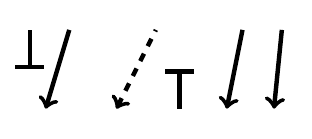
\begin{tikzpicture}
    \draw [ultra thick, |-] (0.4,0.5) -- (0.4,1);
    \draw [ultra thick, <-] (0.6,0) -- (0.9,1);
    \draw [dashed, ultra thick, <-] (1.5,0) -- (2,1);
    \draw [ultra thick, -|] (2.3,0) -- (2.3,0.5);
    \draw [ultra thick, <-] (2.9,0) -- (3.1,1);
    \draw [ultra thick, <-] (3.5,0) -- (3.6,1);
\end{tikzpicture}\\[-0.2em]
My name is Paul .
\end{center}

\end{frame}
%-E--------------------------------------------------------------------------E-%

%-B--------------------------------------------------------------------------B-%
\begin{frame}
\frametitle{Corpora parallèles disponibles}

\begin{itemize} \itemsep0.8em
    \item Europarl~\cite{koehn2005europarl}
    \begin{itemize}
        \item délibérations du Parlement européen disponibles en 21 langues et 
              alignées au niveau de la phrase.
    \end{itemize}
    \item OPUS~\cite{tiedemann2009news}
    \begin{itemize}
        \item \textit{European Medicines Agency documents}, 
              \textit{KDE4 localization files}, Europarl, OpenSubtitles, etc.
        \item \url{http://opus.lingfil.uu.se/}
    \end{itemize}
    \item livres numériques librement disponibles
    \begin{itemize}
        \item \url{http://www.gutenberg.org/}
    \end{itemize}
    \item Wikipédia~: \alert{\fbox{plus comparable que parallèle}}
\end{itemize}

\end{frame}
%-E--------------------------------------------------------------------------E-%


%==============================================================================%
\subsection{Corpus comparable}
%==============================================================================%


%-B--------------------------------------------------------------------------B-%
\begin{frame}[allowframebreaks]
\frametitle{Corpus comparable}

\begin{itemize} \itemsep0.8em
    \item les corpora parallèles sont très couteux et ils ne sont
          disponibles que dans peu de langues/domaines
    \item les corpus dits \textbf{comparables} sont plus répandus
    \item d'après Déjean \& Gaussier~\cite{dejean2002nouvelle}~:
    \begin{itemize}
        \item \og{}Deux corpus de deux langues $l_1$ et $l_2$ sont dits 
              comparables s'il existe une sous-partie non négligeable du 
              vocabulaire du corpus de langue $l_1$, respectivement $l_2$, dont
              la traduction se trouve dans le corpus de langue $l_2$, 
              respectivement $l_1$.\fg{}
    \end{itemize}

    \framebreak

    \item exemple de corpus comparable:
    \begin{itemize}
        \item un ensemble d'articles de journaux dans différentes langues,
              traitant d'une même actualité et à la même époque
    \end{itemize}
    \item applications
    \begin{itemize}
        \item extraction de phrases parallèles~\cite{smith2010extracting}
        \item constitution de dictionnaires bilingues~\cite{rapp1999automatic}
    \end{itemize}
    \item peu (ou pas~?) de corpora comparables disponibles
    \begin{itemize}
        \item Wikipédia, le web multilingue, etc.
    \end{itemize}
\end{itemize}

\end{frame}
%-E--------------------------------------------------------------------------E-%


%==============================================================================%
\subsection{La constitution de corpus}
%==============================================================================%


%-B--------------------------------------------------------------------------B-%
\begin{frame}
\frametitle{La constitution de corpus}

\begin{enumerate} \itemsep0.8em

    \item définir les caractéristiques du corpus~:
    \begin{itemize}
        \item quels sont les phénomènes que l'on souhaite observer~?
        \item quelle est la tâche que l'on souhaite réaliser~?
        \item le corpus doit-il pouvoir être distribué~?
    \end{itemize} 

    \item assembler les unités textuelles
    \begin{itemize}
        \item est-ce que le processus peut être automatisé~?
        \begin{itemize}
            \item e.g.~moissonnage à partir du web (\textit{web scraping})
        \end{itemize}
        \item[$\to$] garder en mémoire la méthodologie utilisée
    \end{itemize}

    \item annotation du corpus (optionnel)
    \begin{itemize}
        \item annoter les unités textuelles (e.g.~\textit{Part-Of-Speech})
        \item créer un référenciel pour l'évaluation (e.g.~termes-clés)
        \item[$\to$] définir des \textit{guidelines} à joindre au corpus
    \end{itemize}

\end{enumerate}

\end{frame}
%-E--------------------------------------------------------------------------E-%

%-B--------------------------------------------------------------------------B-%
\begin{frame}
\frametitle{Étude de cas~: extraction de termes clés}

\begin{itemize} \itemsep0.8em
    \item un corpus pour entraîner et évaluer un système d'extraction de 
          termes-clés
    \begin{itemize}
        \item[$\to$] nature des documents~: \alert{articles}, blogs, tweets, etc.
        \item[$\to$] langue(s) des documents~: anglais, \alert{français}, etc.
        \item[$\to$] source(s) des documents~: lemonde.fr, \alert{wikinews}, 
                     etc.
        \item[$\to$] nombre de documents~: 10, 20, 50, \alert{100}, 1000, etc.
    \end{itemize}

    \item récupération des documents
    \begin{itemize}
        \item automatiser le processus à partir d'un \textit{dump} de wikinews
        \item définir un format pour les documents (XML, txt, etc.)
    \end{itemize}

    \item création d'un référentiel pour l'évaluation
    \begin{itemize}
        \item tâche subjective $\to$ plusieurs annotations par document
    \end{itemize}

\end{itemize}

\end{frame}
%-E--------------------------------------------------------------------------E-%

%-B--------------------------------------------------------------------------B-%
\begin{frame}
\frametitle{Étude de cas~: analyse en dépendances}

\begin{itemize} \itemsep0.8em
    \item un corpus de phrases annotées en dépendances entraîner un 
          \textit{parser}
    \begin{itemize}
        \item[$\to$] langue(s) des phrases~: \underline{\qquad}
        \item[$\to$] source(s) des phrases~: \underline{\qquad}
        \item[$\to$] nombre de phrases~: \underline{\qquad}
    \end{itemize}
    \item récupération des phrases
    \begin{itemize}
        \item[$\to$] automatisée ou manuelle~?
    \end{itemize}
    \item annotation des phrases
    \begin{itemize}
        \item recruter des spécialistes~? définir des \textit{guidelines}~? 
    \end{itemize}

\end{itemize}

\end{frame}
%-E--------------------------------------------------------------------------E-%


%==============================================================================%
\subsection{L'annotation de corpus}
%==============================================================================%

%-B--------------------------------------------------------------------------B-%
\begin{frame}[allowframebreaks]
\frametitle{L'annotation de corpus}

\begin{itemize} \itemsep0.8em

    \item différents niveaux d'annotation~:
    \begin{itemize}
        \item collection de documents, e.g.~regroupement par sujets
        \item document, e.g.~jugement de pertinence en RI
        \item paragraphe, e.g.~découpage thématique
        \item phrases, e.g.~segmentation en phrases
        \item multi-mots, e.g.~détection d'entités nommées
        \item mots, e.g.~tokenization
        \item caractères, e.g.~analyse morphologique
    \end{itemize}

    \item l'annotation d'un point de vue technique
    \begin{itemize}
        \item séparation des annotations du texte
        \item format (e.g.~XML) et encodage standard
    \end{itemize}

     \framebreak

    \item critères de sélection des annotateurs
    \begin{itemize}
        \item spécialistes, e.g.~médecin pour de la RI médicale
        \item natif de la langue, e.g.~évaluation de la grammaticalité
        \item extérieur au projet, e.g.~annotation par les auteurs...
        \item attention au \alert{\textit{crowdsourcing}} !
    \end{itemize}

    \item variabilité des annotations (\textit{consistency})
    \begin{itemize}
        \item résoudre les désaccords par consensus~? 
        \item considérer plusieurs annotations~?
    \end{itemize}

\end{itemize}

\end{frame}
%-E--------------------------------------------------------------------------E-%

%-B--------------------------------------------------------------------------B-%
\begin{frame}
\frametitle{Étude de cas~: annotation de tweets}

\begin{itemize}
    \item détecter la \textbf{polarité} d'un tweet
    \begin{itemize}
        \item annoter un sentiment négatif, neutre ou positif
    \end{itemize}
\end{itemize}

\begin{enumerate} \itemsep5pt
    \item \og{}Décès de Whitney Houston: la vilaine bourde de Sony Music\fg{}
          \only<2>{\alert{$\to$ négatif}}
        
    \item \og{}Interview des \#DaftPunk sur France Inter 1 mois après la sortie 
          de l'album\fg{}
          \only<2>{\alert{$\to$ neutre}}

    \item \og{}Seuls 126\% des marseillais exagèrent.\fg{}
          \only<2>{\alert{$\to$ ?}}
\end{enumerate}

\end{frame}
%-E--------------------------------------------------------------------------E-%


%-B--------------------------------------------------------------------------B-%
\begin{frame}
\frametitle{Un point sur l'encodage}

\begin{itemize} \itemsep0.8em
    \item la lecture/écriture de fichiers textes suppose l'utilisation d'un 
          encodage des caractères
    \begin{itemize}
        \item anglais~: \sout<2>{ASCII}
        \item français~: \sout<2>{ISO-8859-1}
        \item japonais~: \sout<2>{ISO-2022-JP}
        \item etc.
    \end{itemize}

    \Large

    \item<2>[] \alert{$\to$ \textbf{UTF-8}}

\end{itemize}

\end{frame}
%-E--------------------------------------------------------------------------E-%


%-B--------------------------------------------------------------------------B-%
\begin{frame}
\frametitle{Un point sur les méta-données}

\begin{itemize} \itemsep0.8em
    \item une \textbf{méta-donnée} est une donnée servant à définir ou décrire 
          une autre donnée
    \begin{itemize}
        \item e.g.~associer à une donnée la date de création, à une photo les 
              coordonnées GPS du lieu où elle a été prise
    \end{itemize}
    \item le \textit{Dublin Core} est la principale initiative visant à la 
          convergence des éléments de méta-données à utiliser
    \item 15 éléments de description~:
    \begin{itemize}
        \item formels (titre, créateur, éditeur)
        \item intellectuels (sujet, description, langue, etc.)
        \item relatifs à la propriété intellectuelle (droits)
    \end{itemize}
\end{itemize}

\end{frame}
%-E--------------------------------------------------------------------------E-%


